\documentclass{preprint-raac}

% Define directories which contain figures
\usepackage{graphicx} 
\graphicspath{
            {Figures/}
            {Figures/PSF}
            {Figures/Software_Screenshots}
            {Figures/Operating_Principles}
            {Figures/Stability_and_Repeatability}
            {Figures/ML_Exp_Verification}
            } 

% For the author contributions grid
\PassOptionsToPackage{svgnames}{xcolor}
\usepackage{tikz} 
\usetikzlibrary{calc,intersections}
% fonts: you can uncomment this if you want to use pdflatex instead of xelatex (see options in Menu)
%\usepackage{fontspec} 
%\setmainfont{NewComputerModernSans08}

%%
% Preamble: title and author details
\title{Zapit: An Open Source Photostimulation System For Neuroscience}


\author[1,4]{M. Lohse }
\author[1,4]{O. M. Gauld}
\author[1,2,4]{M. Skr\k{e}towska}
\author[1]{P. Vincent}
\author[1]{Q. Pajot-Moric}
%\author[1]{M. V\'{e}lez-Fort}
%\author[1]{S. Weiler}
\author[1]{S. Townsend}
%\author[1]{T. W. Margrie}
\author[1]{C. A. Duan}
\author[1]{A. Akrami}
\author[1]{T. D. Mrsic-Flogel}
\author[1,3]{R. A. A. Campbell}

\affil[1]{Sainsbury Wellcome Centre, UCL}
\affil[2]{University of Cambridge}
\affil[3]{Email: \url{rob.campbell@ucl.ac.uk}}
\affil[4]{These authors contributed equally}
%% Corresponding author
\corrauthor{R. A. A. Campbell}

%% Abbreviated author list for the running footer
\runningauthor{Lohse, Gauld, Skr\k{e}towska et al.}

\addbibresource{references.bib}

\begin{document}

\maketitle


%%
% Abstract and keywords
\begin{abstract}
Optogenetic tools are indispensable for understanding the causal neural mechanisms giving rise to animal behaviour. 
While optogenetic actuators provide millisecond-precision control over genetically defined neural populations, successful optogenetics experiments also critically depend on associated optical hardware for targeted light delivery. 
% Optic-fibres are suitable for certain experiments, yet fibre implantation can be invasive and limits flexibility of spatial targeting. 
% Precise spatiotemporal control over light delivery is essential as behavioural tasks can engage distributed neural circuits with complex dynamics. 

% To address this, galvonometer-based laser-scanning optogenetic systems have been used to allow flexible inactivation of distributed cortical areas, through the intact skull and without the need of optic fibers. 
% These approaches centre on controlling hardware to steer a small laser-spot to user-defined locations on the dorsal surface of the cortex of mice, which selectively activates or inhibits neurons in the local illuminated region. 
% While experimentally powerful, bespoke laser-scanning photostimulation systems can be technically challenging and expensive to build, and at present no open source solution is available. 
Implanted optical fibres are 
In contrast, galvonometer-based laser-scanning optogenetic systems facilitate far greater flexibility for targeting distributed cortical areas. Yet no open source systems are available at present, and building such bespoke photostimulation systems can be technically challenging and expensive to build.

Here we present Zapit, a complete open source hardware and cross-platform software system for spatio-temporally precise laser-scanning optogenetics experiments in head-fixed mice. 
We provide step-by-step instructions on how to build, calibrate and design experiments using the Zapit system, and present quantification of optical system performance, as well as results from proof-of-principle cortical photoinhibition experiments in awake behaving mice.

\keywords{Optogenetics, Neuroscience, Software Tool, Optics, Open Source}
\end{abstract}

%% 
% Intro, Results, and Discussion in separate files
\section{Introduction}
\label{sec:introduction}

 
With an increasing interest in systems neuroscience came improvements in methods of observing neuronal activity across multiple regions. Advances in techniques such as wide-field imaging (refs) and ephys recordings (refs) necessitated development of effective and flexible techniques of causal investigation on a matching scale.
Since its invention, optogenetics has become the preferred experimental tool for manipulating neural activity in systems neuroscience due to its high temporal precision and genetically-constrained impact of modulation [REF]. 
Initially, light delivery was achieved via chronically implanted fibres (refs).
Whilst this approach allows the animal to move around its environment, only a small, fixed, number of stimulation sites in sufficiently distant configuration (due to the physical size of implants) is possible. 
Tapered fibres are one way to solve this problem, as they allow for targeting multiple regions along the fibre length (REF). 
In mice it is feasible to perform targeted photo-stimulation of dorsal cortex through the intact skull. 
This idea made it possible to address questions posed by an increasing number of studies describing patterns of wide-field Ca\textsuperscript{++} activity (). 

Optogenetic photostimulation through the exposed skull in head-fixed animals allows for flexibly targeted, programmatic, stimulation.
The method can be as simple as a fibre optic mounted on motorized micro-drives (\cite{Zatka-Haas2021SensoryDecision}) or as elaborate as imaging a digital micromirror array onto the exposed cortex [Allen, 2017, other refs].
A particularly fruitful approach has been to use  galvanometric scan mirror (galvos) to target a focussed laser beam (\cite{Guo2014FlowMice,Li2016RobustPlanning,Heindorf2018MouseFeedback,Inagaki2018Low-dimensionalCortex, Keller2020FeedbackCortex,Voitov2022CorticalMemory,Pinto2019Task-DependentRegions,Coen2021FrontalModalities,Pinto2022MultipleCortex}). 
Whilst the galvo approach is both powerful and relatively affordable, there remains no well packaged open source solution for implementing it.

The last decade has seen widespread adoption of open source hardware tools in neuroscience, such as Open-Ephys (\cite{Siegle2017OpenElectrophysiology}), the `Pulse-Pal' pulse generator (\cite{Sanders2014ABehavior}), the `Stimjim` programmable electrical stimulator (\cite{Cermak2019Stimjim:Stimulation}), as well as countless designs for light-sheet and multi-photon microscopes. 
Surprisingly there exists no equivalent project for random access photostimulation in head-fixed animals.
Anyone wishing to implement such a system needs to build it from the ground up, which is time consuming and requires as solid understanding of optics, data acquisition, and programming.
Here we present `Zapit', an open source galvo-based photostimulator, which we hope fills this gap, by providing a standarized, affordable and easily accessible version of this useful method.

‘Zapit’ is the combination of an open-source galvo-based hardware design and an associated software ecosystem for calibration and stimulus delivery. 
The hardware was designed with the intention of making it as compact as possible so it can fit into tight behavioural enclosures. 
Relative low cost and short lead times ensure it remains accessible.
Our system is flexible regarding inactivation protocols, from single points to multiple areas targeted bilaterally. 
We demonstrate how Zapit allows for fast and easy integration of targeted photostimulation into a variety of behavioural tasks.
\section{Results}

\subsection{Operating principle}
Zapit is best thought of as a software-based solution for galvo-based photo-stimulation. 
Whilst we provide hardware designs (see below), there is no fixed design that is required to work with the software.
A variety of hardware designs can work and Zapit is flexible enough to take this into account. 

Here we implemented a hardware design similar to that used in \citet{Pinto2022MultipleCortex}.
A 470~nm laser is fed into an XY galvo scan block then is pointed down to the animal via a dichroic fold mirror.
A 100~mm achromatic lens focuses the beam onto the sample.
This lens doubles as an objective: imaging the sample and any excited green fluorescence onto a camera via a 50~mm tube lens (Fig.~\ref{fig:operating_principle_01}A).
The galvo waveforms are shaped to make them near inaudible, but nonetheless we designed a sealed enclosure for the scanners (Fig.~\ref{fig:operating_principle_01}B).

The Zapit software comprises of a user-friendly GUI for performing the two critical alignment steps. 
\textbf{1.} Aligning the scanners with the camera, enabling the beam to point accurately to any desired location in the image. 
\textbf{2.} Mapping stereotaxic coordinates onto the exposed skull.  
Calibration takes about a minute and, once calibrated, the system will place the beam in any desired location defined by stereotaxic coordinates. 

Once calibrated, a simple API allows the user to integrate stimulation into an experimental paradigm. 
The system currently supports stimulation of either one or two points in a given trial (extending it to more points is planned for the near future). 
In any given trial the laser spot either sits on one point and flashes on and off at 40~Hz or it goes back and forth between two spots in a 50/50 duty cycle illuminating each at 40~Hz. 
The location(s) of the beam in each stimulus condition is defined in stereotaxic coordinates.
There is a ramp down in intensity at trial end to avoid rebound effects. 
An optional blue LED masking light runs in synchrony with the laser.

\begin{figure}[h]
\centering
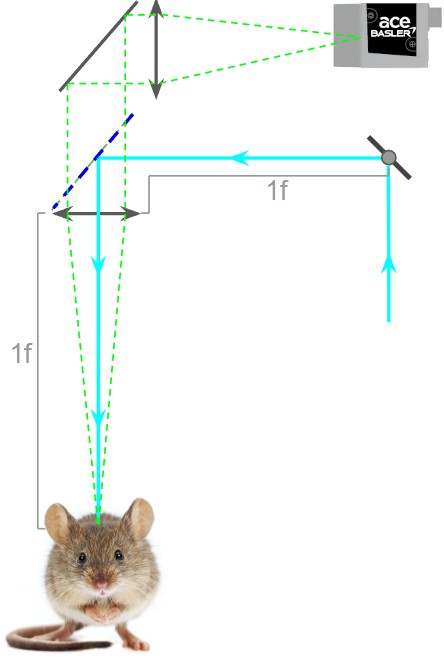
\includegraphics[width=0.325\textwidth]{Figures/Operating_Principles/Zapit_operating_principle_light_path.jpg}
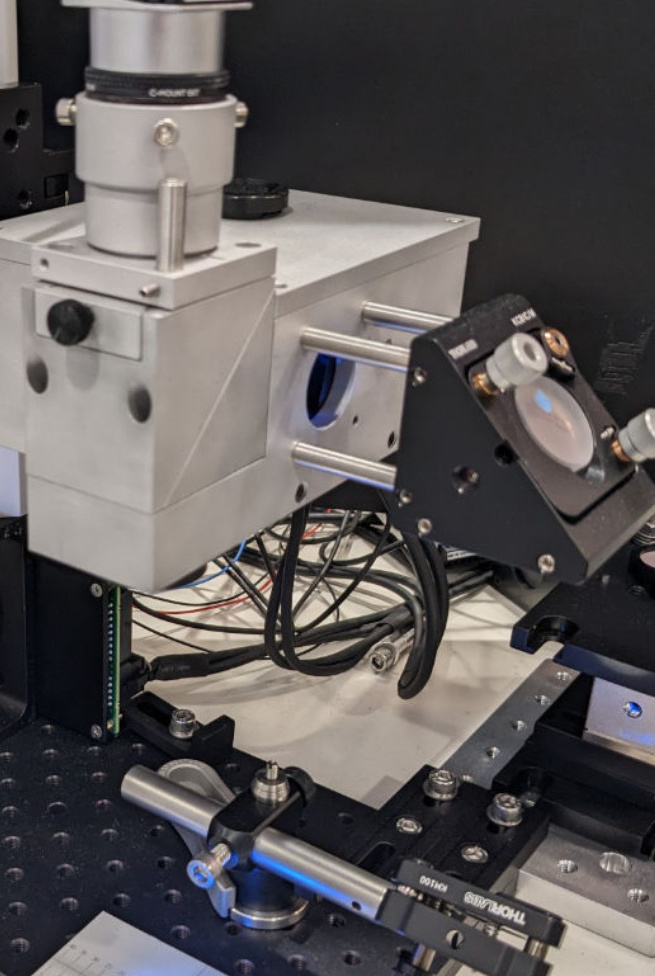
\includegraphics[width=0.325\textwidth]{Figures/Operating_Principles/Zapit_example_system_photo.jpg}
\caption{\textbf{A}. Optical path schematic.
A laser beam (blue) is directed using a pair of scan mirrors then focused through a lens and onto the skull surface via  dichroic mirror. 
The lens is located 1f from the scanners so that it behaves telecentrically. 
The dichroic allows the sample to be imaged on a camera via a tube lens
The beam location on the skull surface is visible due to autofluorescence. 
\textbf{B}. A photographed of an assembled system in a custom-built aluminum enclosure.}
\label{fig:operating_principle_01}
\end{figure}


\subsection{Hardware Design}

Details on the enclosure. 
Details on the Thorlabs CAD model.
Theoretical laser spot size is xx~$\mu m$.
PSF: theory. predicted. 

\begin{figure}[h]
\centering
\includegraphics[width=0.6\textwidth]{example-image}
\caption{A. Optical path schematic. B. Maybe a Zemax diagram. C. Photo of the system. D. Photo of the system.}
\label{fig:hardware01}
\end{figure}

\subsection{Software Design}
Explain how the software achieves the above.
A GUI allows specifying of points in stereotaxic coords and hence creation of settings files with respect to the Allen Atlas (Fig.~\ref{fig:software01}). 
Describe where this came from: the cortex lab and is that used by IBL.
Another GUI is used to calibrate the scanners such that they are able to point to locations in the image defined by the user. 
A second step defines the position of the skull in the FoV and hence previously specified stereotaxic coords can be overlaid onto the sample. 
The GUI has tools to allow visual confirmation of the scan and sample calibration steps (Fig.~\ref{fig:software02}).  

\begin{figure}[h]
\centering
\includegraphics[width=0.6\textwidth]{example-image}
\caption{Screenshot of stim config editor}
\label{fig:software01}
\end{figure}


\begin{figure}[h]
\centering
\includegraphics[width=0.6\textwidth]{example-image}
\caption{A. Screenshot of scanner calibration process. 
B. Screenshot of sample calibration process.}
\label{fig:software02}
\end{figure}


\subsection{Calibration}

The user initiates an automatic calibration procedure that maps the galvo control signals to pixel locations in the image. 
A simple two-click interface allows the user to map stereotaxic coordinates onto the image space. 

\subsection{Running Experiments}
Once the system is calibrated and a stimulus configuration file is loaded, it becomes possible to run an experiment.
There is an API available in MATLAB. 
The \texttt{sendSamples} command defines which stimulus will be presented next. 
By default the system queues the stimulus and waits for a TTL trigger before presenting it.
The \texttt{stopOptostim} command stops the stimulus whilst ramping down laser power over a user-defined time period.
If an `experiment directory' is defined in Zapit, \texttt{sendSamples} will write there a log file listing each stimulus presentation.
Control trials are possible where the galvos move and the masking light is on but the laser is off.

\lstinputlisting[language=MATLAB]{code_snippets/basic_api_example.m}

\subsection{Control via Python}
The `zapit-Python-Bridge' (installed via PyPI) provides access to the MATLAB API via shared memory. 
The user must start Zapit in MATLAB and conducted the scanner and sample calibration steps. 
All subsequent operations can be done via Python with commands that resemble those used in MATLAB.
For example:

\lstinputlisting[language=Python]{code_snippets/one_stim_example.py}

Zapit must remain running in MATLAB throughout. 


\subsection{Other languages}
Users wishing to use a different programming language must re-implement the \texttt{sendSamples} and \texttt{stopOptoStim} commands. 
This is straightforward and We provide minimal examples in the main Zapit repository to assist with this. 



\subsection{Validation}
\subsubsection{Scanner calibration accuracy}
Accuracy with which beam points to target in microns.
How the hell do we measure this? Using the camera? 
But then how accurate is our estimate of where the beam actually went? 
I guess we can show many points indicating where the beam went over many trials. 
That will show up bias.
But spread around the target location could be due to pointing errors or it could be due to errors in locating the beam. 
We can correlate with the galvo feedback waveforms and so know the error.
(Fig.~\ref{fig:validation01}A).

\subsubsection{Repeatability and Stability}
Have it run, say, 1000 trials of two locations quite far apart and record the command waveforms, galvo feedback, and beam intensity (Fig.~\ref{fig:validation01}B). 
Overlay these and show consistency over long periods of time and many trials. 
Feedback signals show us that the beam has arrived at the target location before being switched back on. 

\begin{figure}[h]
\centering
\includegraphics[width=0.6\textwidth]{example-image}
\caption{A. Scanner accuarcy
B. Repeatability and stability.}
\label{fig:validation01}
\end{figure}


\subsubsection{Suitability}
Measure laser power over the FOV and confirm it is the same everywhere (IT IS).

\section{Discussion}

Zapit is a complete and accessible solution for head-fixed scanner-based optogenetics. The components are commercially available, and the modular system is flexible enough to accommodate a diversity of experimental needs. The \href{https://github.com/Zapit-Optostim/zapit}{Github} repository contains complete build instructions, parts lists, and visual aids: no prior expertise is required for implementation. The  software is fully documented and will be continually maintained and updated by developers and experimentalists. Known software and hardware issues are actively raised and resolved through \href{https://github.com/Zapit-Optostim/zapit/issues}{Github} issues and community discussions. 

Zapit produced robust behavioral effects across a variety of experimental protocols and brain regions with VGAT-ChR2 mice. We validated the efficacy of inactivation in this mouse strain with simultaneous electrophysiology recordings and demonstrate that the effective radius of inactivation depends on the laser power used, but was \textasciitilde{}1~mm at powers for which we observed significant behavioral perturbations. However, with finer spatial sampling and large trial numbers, it is possible to observe distinct behavioral effects at sites separated by less than 1 mm.

There are other effective approaches for rapid programmatic photostimulation in head-fixed behavioral tasks: those based on digital micro-mirror devices (DMDs \cite{Chong2020ManipulatingPerception, Russell2022All-opticalMice, Gauld2024APerception}) or spatial lights modulators (SLM). DMD-based solutions, such as the \href{https://www.mightexbio.com/polygon/}{Mightex Polygon}, provide a faster pattern-switching time but due to light loss, these systems require \textit{\textasciitilde{}100 times} more laser power than Zapit to cover the mouse dorsal cortex. SLM-based solutions are more light efficient, but devices with high resolution are very expensive and are slower than DMDs. Therefore, Zapit's scanner-based approach provides the most cost-effective and compact solution for the majority of optogenetic experiments. 

\subsection{Practical considerations when using Zapit}
\subsubsection{Surgical procedures} 
To maximize targeting flexibility and accuracy, we recommend a head-fixation device that provides an unobstructed view of the entire dorsal surface of the skull, and marking structural reference points during surgery. We further recommend a thin layer of transparent glue (\cite{Zatka-Haas2021SensoryDecision, Coen2023MouseDecisions}) or `bone' cement (200-300~$\mu m$ thick) to protect the skull as thicker layers of cement (0.5-1~mm) may reduce the efficacy of behavioral effects. For general details of \textit{in vivo} surgical and behavioral procedures in head-fixed mice we direct the reader to existing resources (e.g. \cite{Guo2014FlowMice, Guo2014ProceduresMice} ). 

\subsubsection{Laser and power selection}
Zapit is compatible with any laser source with fast analog power modulation. Each setup will have unique experimental constraints but, as a guideline, we recommend using 1-2~mW time-averaged light power when using VGAT-ChR2 mice. We consistently see strong behavioral effects at these powers, and spatiotemporal resolution comparable with many other studies. Regular power measurements at the sample are critical to ensure stability and reproducibility. At 2~mW time-averaged power, and with expected light loss of around 50\% due to the skull and bone cement (\cite{Guo2014FlowMice}), heating of the neural tissue should be minimal (\cite{Stujenske2015ModelingOptogenetics}). Nevertheless, \textit{post-hoc} histological analysis is strongly recommended to confirm opsin expression and assess tissue integrity.

\subsubsection{Targeting precision}
With transgenic lines expressing opsin brain-wide (including VGAT-ChR2 mice), stimulation with high laser powers (e.g. 4~mW or above) may cause off-target behavioral effects due to light-scatter laterally and axially through cortex (\cite{Li2019SpatiotemporalCircuits,Babl2019TheInterneurons}). Ideally, laser parameters including power, duration and ramp-down should be informed by electrophysiological recordings and/or modeling of light propagation through biological medium (\cite{Yona2016RealisticApplications}). If limiting the impact of light dispersion is critical, opsins can be expressed via targeted viral injections. Under these conditions, expression can be restricted to highly localized circuits, genetically and anatomically defined subpopulations and sub-cellular compartments, and verified using \textit{post-hoc} histology.

\subsubsection{Sensory confounds}
Fast movements of galvo-mirrors generate auditory cues that can influence behavior, and we therefore recommend including moving the galvo-mirrors on all trials, including those where the laser power is 0~mW. The galvo drive waveforms are shaped to reduce noise emission, and the scanner unit can also be enclosed sound-attenuating housing to further mitigate these effects. To accurately interpret optogenetic behavioral effects, it is also critical to mask the mouse's ability to see the laser, whether through internal or external retinal stimulation \cite{Weiler}. We recommend masking laser-emitted light with color-matched LEDs placed above the mouse on every trial, matched to the stimulation profile of the laser (e.g., 40~Hz sinusoid). Extra caution should be taken when using longer wavelengths which easily propagate through brain tissue to the retina, and can be more difficult to mask (\cite{Danskin2015OptogeneticsArtifact}). Sensory confounds can also be addressed through repeated experiments and analyses in control animals that do not express the stimulated opsin (\cite{Gauld2025AActions}).

\subsubsection{Target region selection and interpretation} 
A major advantage of Zapit is the capacity to perform unbiased sampling of causal effects across the entire dorsal cortex. However, skull curvature and thickness should be considered, particularly in more lateral cortical regions. Differences in opsin expression due to tropisms in viral vectors or transgenic lines can also influence results and further experiments are required to determine whether observed effects are a direct result of regional inactivation, or derive from downstream brain regions (\cite{Wolff2018TheManipulations, Allen2017ApplicationSignaling}).

\subsection{Good practice: measures to report when using Zapit}
We encourage Zapit users to report a minimal set of standardized parameters to aid replication, comparability, and consistency across experiments and laboratories:

\begin{itemize}
    \item Average light power
    \item Peak light power
    \item Stimulation frequency and profile (e.g. 40~Hz sinusoid), and duty cycle
    \item Laser stimulation and ramp-down duration
    \item Color and frequency of masking light (if used)
\end{itemize}

\subsection{In Closing}
We hope Zapit is a tool that will grow and find uses outside of our institute and specialties. Potential new users are welcome to contact us for assistance in building or setting up the system. 

\section{Methods}

\subsection{Wavelength Validation Experiments}

\subsubsection{Subjects}
All experiments were performed on 15-20 weeks old C57BL/6 or B6.129P2-Pvalbtm1(cre)Arbr/J (PV-Cre) male mice in accordance with the UK Home Office regulations (Animal (Scientific Procedures) Act 1986), approved by the Animal Welfare and Ethical Review Body (AWERB; Sainsbury Wellcome Centre for Neural Circuits and Behavior) and in compliance with ARRIVE guidelines.

\subsubsection{Surgical procedures}
Mice were anesthetized under isoflurane (2\%-5\%), carprofen or meloxicam was administered (5mg/kg or 1-2 mg/kg, respectively; s.c.) and eyes were protected with eye gel Lubrithal (Dechra).
Mice were then fixed to a stereotaxic frame and their body temperature maintained at 37-38 °C. They were implanted with a head plate fixed to the skull using Histoacryl (Braun Medical) and C\&B Metabond (Sun Medical). 
Additionally, we added a layer of black dental cement (Kemdent) on top of the Metabond.
For the implantation of the optical fiber, a craniotomy of $\sim$1~mm radius was drilled over the region of interest using a 0.3~mm burr dental drill (Osada Electric).  The optical cannula (Newdoon 200 microns, 1.5 mm, NA 0.37) was then inserted 550 um from the pial surface into the cortex and fixed to the skull using light-cured resin dental cement Relyx Unicem 2 (3M).
The skull was then covered with C&B Metabond and subsequently covered with black cement. Animals were allowed to recover for at least 48 hr.
The implantation of the optical fiber above the intact skull followed the same procedure, but omitting the drilling of a craniotomy.
On the day of extracellular recording (after habituation to head-fixation that typically took 2-3 sessions of 30 minutes each), animals were anesthetized under isoflurane (2\%-5\%), their whiskers trimmed (to 2 to 5~mm long) and a small craniotomy (1 x 1 mm) was drilled over the brain region of interest using a 0.3~mm burr dental drill. The craniotomy was sealed with silicon Kwik-Cast (World Precision Instruments) and the animals were allowed to recover for at least 2 hr prior to recording.

\subsubsection{Experimental setup}
The visual stimulus consisted of two laser projectors (60 fps; MP-CL1A, Sony) projecting on two rear-projection screens.
The two rear-projection screens were positioned in front of the animal, 5 cm from each eye at a 90 degree angle to each other (visual field covered: ~75 of elevation and ~270 azimuth).
In ambient light experimental conditions, isoluminant gray or drifting gratings (Spatial Frequency = 0.02 cpd; Temporal Frequency = 2 Hz) were presented on the rear-projection screens using the Psychophysics Toolbox (\cite{Brainard1997TheToolbox.}).
In addition, an LED strip surrounding the experimental setup (Goove) was turned on. In complete darkness conditions, the screens and LED strip were turned OFF and two small light shields were positioned in front of the animal’s eyes.
In both light and dark conditions, a light shield was positioned at the base of the optical fiber.
A Faraday cage was built around the experimental apparatus to provide both electrical noise isolation and pitch darkness.

\subsubsection{Extracellular recordings}
The silicon probe (IMEC, Belgium) was first coated with DiI (Molecular Probes, Thermo Fisher Scientific).
The probe was then positioned perpendicular to the brain surface and the tip inserted 2000~µm from the pial surface using micro-manipulators (Luigs and Neumann).
The probe was allowed to settle for approximately 30 minutes before recordings. The reference electrode consisted of a Ag/AgCl wire positioned close (<2~mm) to the craniotomy.
The craniotomy, as well as the reference wire, were covered by Agar 3\% prepared in cortex buffer (NaCl 125~mM, KCl 5~mM, Glucose 10~mM, HEPES~10 mM, CaCl2 2~mM, MgSO4 2~mM, pH~7.4). 
The Agar was then submerged by the cortex buffer.
Neuropixels Phase 3A probes were connected to a dedicated FPGA card (KC705, Xilinx). 
SpikeGLX v20180525-phase3A (\texttt{github.com/billkarsh/SpikeGLX}) were used to acquire data. Data were filtered at 300~Hz during or after acquisition.


\subsubsection{Laser stimulation}
An optical cord (Newdoon MM200/220, NA 0.37) was used to provide the laser stimulation (637~nm: Thorlabs S4FC637; 594~nm: Coherent Obis 594~nm LS 40~mW Laser, Fiber Pigtail, FC; 473~nm: Thorlabs S4FC473).
In pitch darkness and ambient light with gray screens, 40 laser stimulations were presented in 5 blocks of 8 stimulations. 
Within each block, each laser stimulation lasted 2~s and was separated by 2~s.  
Each block was separated by 54~s.
In ambient light experimental conditions with drifting gratings, 80 laser stimulations were presented in 10 blocks of 8 stimulations. Within each block, each laser stimulation started 1 second after the onset of drifting gratings, and lasted for 2~s separated by 2~s. Each block was separated by 54~s.

\subsubsection{Probe localisation}
Following silicon probe recordings, animals were deeply anesthetized and transcardially perfused with cold phosphate buffer (PB, 0.1 M) followed by 4\% paraformaldehyde (PFA) in PB (0.1 M) and brains left overnight in 4\% PFA at 4 °C. 
Brains were then embedded in 4\% agar and imaged using serial two-photon tomography (\cite{Mayerich2008Knife-edgeBrain,Ragan2012SerialImaging,Winnubst2019ReconstructionBrain.}), using  BakingTray (\cite{Campbell2020BakingTray}), a custom wrapper around ScanImage (Vidrio Technologies, \cite{Pologruto2003ScanImage:Microscopes.}).
Images were acquired as tiles with 5-7~µm axial sampling and 2.27 x 2.27~µm pixels, and stitched using StitchIt (\texttt{https://github.com/SainsburyWellcomeCentre/StitchIt}, \cite{Han2018TheCortex.}).
Images were then registered to the Allen Mouse Brain Common Coordinate Framework version 3 (CCFv3, 25~µm resolution; \cite{Wang2020TheAtlas}) using brainreg (\cite{Tyson2022AccurateImages,Niedworok2016AMAPData}).⁠
The atlas data were provided by the BrainGlobe Atlas API (\cite{Claudi2020BrainGlobeAtlases}).
Probe tracks were confirmed by DiI fluorescence and were traced using brainreg-segment (\cite{Tyson2022AccurateImages}).

To refine the localisation of the probe, we used electrophysiological information. 
In primary visual cortex (VISp) recordings, we determined the middle of layer 5 using the depth profile of the high-frequency LFP power (\cite{Senzai2019Layer-SpecificMouse}).
For each non-reference channel on the probe, the average power in the frequency range 500~Hz-5~kHz was computed (MATLAB, The MathWorks Inc., \texttt{bandpower} function). 
Each bank of electrodes (4 for Neuropixels Phase 3A) was separated, and the power profile was linearly interpolated at 1~µm resolution along the bank before being smoothed with a 100~µm sliding window.
The profiles along each bank were averaged and the location, in the cortex, of the peak in this depth profile was chosen as the middle of layer 5.
To determine cortical depth in VISp of isolated single units when pooling across animals, we first determined the layer in which the unit occurred.
We then calculated the relative depth of the unit in that layer in that animal (value between 0 and 1).
The boundaries of each layer were then averaged across mice and the unit was positioned within its layer at the relative depth determined from the previous step.

\subsubsection{Spike sorting and analysis}
Spike sorting and unit quality control were performed using a fork of the \texttt{ecephys\_spike\_sorting pipeline} 
(\cite{Siegle2017OpenElectrophysiology}) modified for SpikeGLX data 
(\texttt{github.com/jenniferColonell/ecephys\_spike\_sorting}; for Neuropixels Phase 3A recordings commit \texttt{55ff943892577cee497e28dd6a201f4f101b0777}; Velez-Fort et al., 2023).
Raw data acquired with SpikeGLX were filtered with CatGT (\texttt{billkarsh.github.io/SpikeGLX/\#catgt}) and Kilosort2 was run.
For single unit analysis only clusters deemed “good” were considered (\texttt{github.com/MouseLand/Kilosort}; commit \texttt{2a399268d6e1710f482aed5924ba90d52718452a}).
Double counted spikes were removed (\cite{Siegle2017OpenElectrophysiology}) and finally, waveform and quality metrics were computed. 
Only clusters of spikes that had an ISI violation metric (\cite{Hill2011QualitySignals}) less than 0.15, amplitude cutoff metric (\cite{Siegle2017OpenElectrophysiology}) less than 0.1, maximum drift less than 80~µm, and isolation distance (\cite{Schmitzer-Torbert2005QuantitativeRecordings}) greater than 20 were considered putative single-units and examined for further manual curation.  
All units (wide- and narrow-spiking units) were pulled for further analysis.

Firing rates during baseline and laser stimulation periods were calculated on a trial-by-trial basis.
Spike trains were convolved with a 5 millisecond-wide Gaussian window, to get a continuous spike rate.
For each laser stimulation, 2 windows of interest of 200~ms each were taken into consideration: immediately before (baseline) and immediately after laser stimulation onset.
The mean of the spike rate trace during baseline and laser stimulation windows was then taken.
A single unit was considered significantly modulated by laser stimulation, if the p-value from a Wilcoxon signed-rank test performed on baseline and stimulus firing rates was less than 0.05.
At a neuronal population level, 2 windows of interest of 100 ms each were taken into consideration: a baseline window immediately before laser stimulation and a laser stimulation window that started at the respective average onset latencies for 637, 594, and 473~nm recorded in ambient darkness.
A population of neurons were deemed significantly modulated by laser stimulation if the p-value from a Wilcoxon signed-rank test performed on baseline and stimulus firing rates was less than 0.05.
\section{Author Contributions}
\tikzset{
    tile/.style = {
        align=center,
        minimum size=6mm,
        anchor=north west,
    },
    col header/.style={
        tile,
        anchor=north west,
        yshift=-1mm,
        rotate=45,
        inner sep=0,
        outer sep=0,
    },
    row label/.style={
        tile,
        anchor=north east,
        inner sep=0,
        outer sep=0,
        xshift=3mm,
    },
    legend line/.style={
        anchor=north west,
        inner xsep=0,
        inner ysep=2mm,
        outer sep=0,
    },
}

% define the intensity levels here
\def\hi{100}
\def\mid{50}
\def\lo{20}

% and the 100% intensity color here, which will blended to white
\colorlet{tilecolor}{green!10!orange}

\begin{tikzpicture}[scale=0.6]

    % column labels
    \foreach \a [count=\n] in {
        M.L.,
        O.M.G.,
        M.S.,
        A.M.,
        C.B., 
        J.L,
        G.N.,
        Q.PM.,
        S.T.,
        P.V.,
        A.A.,
        C.A.D.,
        J.E.H.,
        T.D.MF.,
        P.C.,
        R.A.A.C.,
    } {
        \node[col header] at (\n,0) {\a};
    }

    % row labels
    \foreach \a [count=\i] in {
        Prototype hardware design,
        Prototype software design,
        Final hardware design,
        Final software design,
        CAD \& machining,
        Behavioral validation experiments,
        Writing---Original Draft,
        Writing---Reviewing and Editing,
        Funding acquisition,
    } {
        \node[row label] at (0,-\i) {\a};
    }

    \foreach \y [count=\n] in {
        {\mid,0,\hi,0,0,0,0,0,0,\hi},  %hardware prototype
        {0,0,\hi,0,0,0,0,0,0,\hi},     %software prototype
        {0,0,0,0,0,\lo,0,0,0,\hi},     %hardware
        {0,0,0,\lo,\lo,0,0,0,0,\hi},   %software
        {0,0,0,0,0,\hi,0,0,0,0},       %CAD
        {\hi,\hi,\lo,0,0,0,0,0,0,0,0}, % Behav valid
        {\hi,\hi,\mid,0,0,0,0,0,0,\hi}, %Writing: draft
        {\mid,\mid,\mid,\mid,\mid,\mid,\mid,\mid,\mid,\mid}, %Writing: edits
        {\hi,0,0,0,0,0,\hi,\hi,\hi,0},  % Funding
    } {
        % heatmap tiles
        \foreach \x [count=\m] in \y {
            \node[fill=tilecolor!\x!white, tile, text=white] (tile) at (\m,-\n) {};
        }
    }

    % description below heatmap 
    %\node [legend line] at (1, 0 |- tile.south) {*, $^\dagger$ these authors contributed equally};

\end{tikzpicture}

%% 
% Close
\paragraph*{Acknowledgments}
We thank Andy Peters for providing us with a MATLAB script for displaying a top-down view of the Allen Atlas in stereotaxic coordinates, and inspiring us with the Neuropixels Trajectory Explorer (\href{10.5281/zenodo.7043459}{10.5281/zenodo.7043459}).
Dale Elgar from \href{https://www.cosys.org.uk/}{COSYS Ltd.} did most of the enclosure design. 
Graeme McPhillips at the SWC Electronics Core Facility provided advice on construction of the control electronics enclosure. 


\paragraph*{Data Availability Statement}
This project is developed entirely in the open: all code is available at \href{https://github.com/Zapit-Optostim}{github.com/Zapit-Optostim}.
Data available on request.


\printbibliography
\end{document}